\section{Simulation Validation}
To validate the chosen simulation approach, identical system perturbances were performed in the GE Energy Positive Sequence Load Flow (PSLF) Dynamic Subsystem (PSDS) and PSLTDSim.
%The output data was then compared in MATLAB.
Frequency is compared to validate the single system frequency assumption calculated by PSLTDSim, and governed generator mechanical power is compared to validate governor action.

To simplify the comparison of frequency data from PSDS to LTD, a single weighted frequency based on generator inertia was calcualted using (\ref{eq: f_weighted}) and (\ref{eq: Hsys}).
\begin{align}
f_{w} &= \sum_{i=1}^{N} f_i \dfrac{H_{PU, i} M_{base, i} }{H_{sys}}  \label{eq: f_weighted}\\
\text{where } H_{sys} &= \sum_{i=1}^{N} H_{PU, i} M_{base, i}  \label{eq: Hsys}
\end{align}% This explanation may be unnecessary for IEEE...
Due to the different time steps, when calculating the difference between PSDS and LTD, multiple PSDS values have the same held LTD value subtracted from them. 
For instance, any PSDS($t = 3.x$) would have the LTD($t = 3$) value subtracted from it for comparison.

% Something about an individual difference not mattering as much as the general difference, therfore all ltd psds comparisons are plotted as a single color.

%-------------------------------------------------------------------------------------
\subsection{The MiniWECC System}

The power system used for validation and valve travel experiments, the miniWECC shown in Fig. \ref{fig: miniWECC}, is a 120 bus 34 generator system created in PSLF.
All governors in the miniWECC are modeled with the tgov1 which enabled easier validation.
Further details about the creation and use of the miniWECC may be found in \cite{trudnowski2012, sandia2015, RJminiWECC}.

\begin{figure}[!ht]
	\centering
	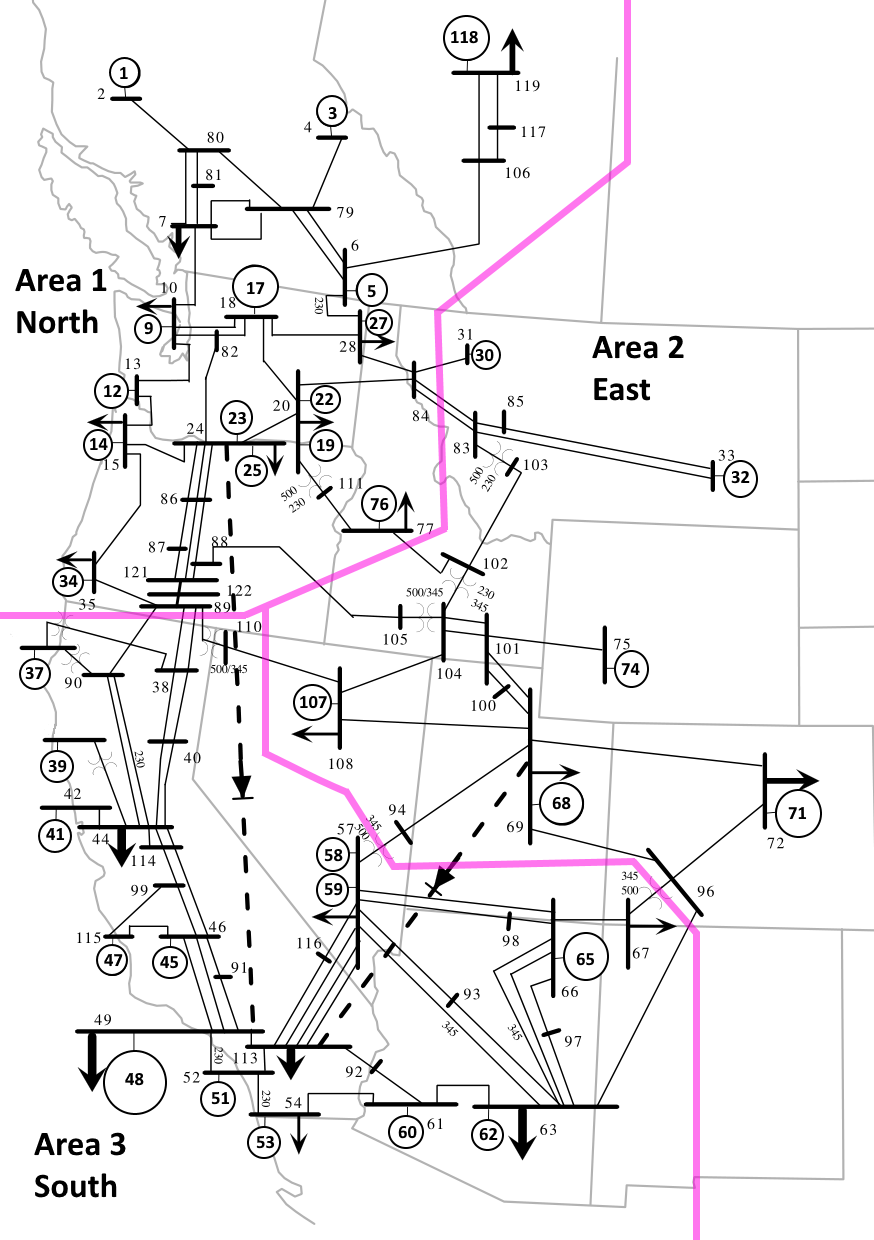
\includegraphics[width=.65\linewidth]{figures/miniWECC_split03}
	\caption{MiniWECC System adapted from \cite{RJminiWECC}.}
	\label{fig: miniWECC}
\end{figure}

%`````````````````````````````````````````````````````````````````````````````````````
\subsubsection{Load Step Results}
A 400 MW load step was simulated to occur at 2 seconds.
As shown in Fig. \ref{fig: stepFcomp}, all individual PSDS frequencies begin to oscillate after the perturbance while the weighted PSDS frequency appears to follow the general center of oscillation. The LTD system frequency is less oscillatory than the weighted frequency with only minor differences between the two. Fig. \ref{fig: rampFdif} quantifies these differences.

\begin{figure}[!t]
	\centering
	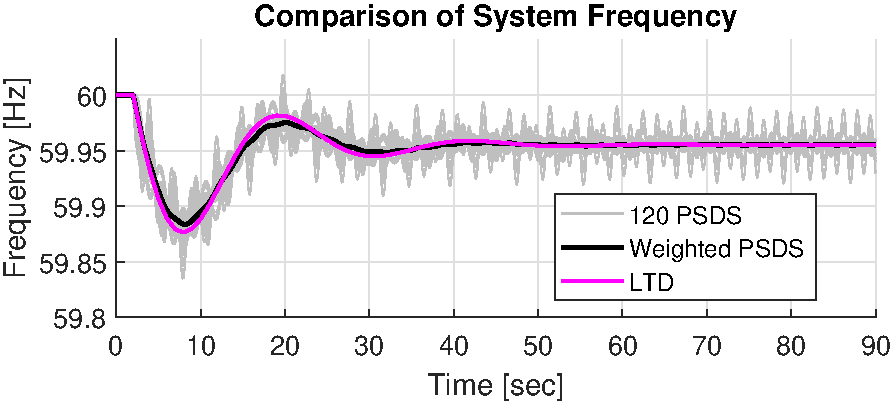
\includegraphics[width=\linewidth]{figures/miniWECC3ALTDstepF3}
	\caption{Comparison of frequency during load step.}
	\label{fig: stepFcomp}
\end{figure}

\begin{figure}[!t]
	\centering
	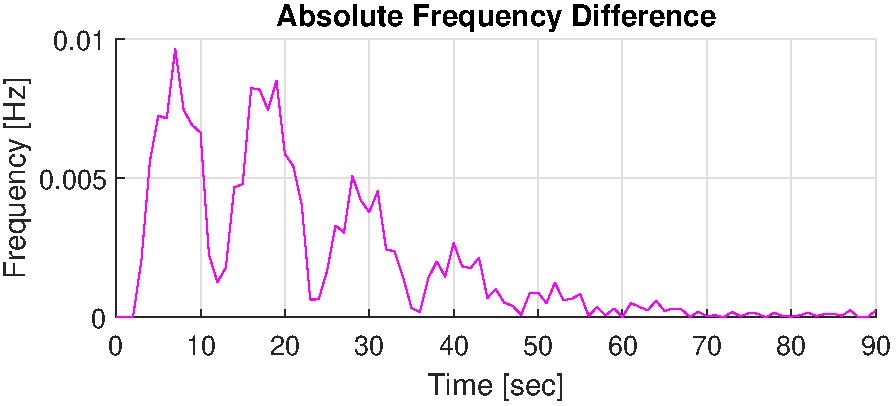
\includegraphics[width=\linewidth]{figures/miniWECC3ALTDstepRelF}
	\caption{Absolute difference of weighted frequency during load step.}
	\label{fig: stepFdif}
\end{figure}

When comparing mechanical power output in Fig. \ref{fig: stepPmdif}, large MW differences can be seen, however, the percent difference data in Fig. \ref{fig: stepPmPercentdif} shows results less than 5\% max difference, and an average percent difference of less than $\approx$0.5\%.

\begin{figure}[!ht]
	\centering
	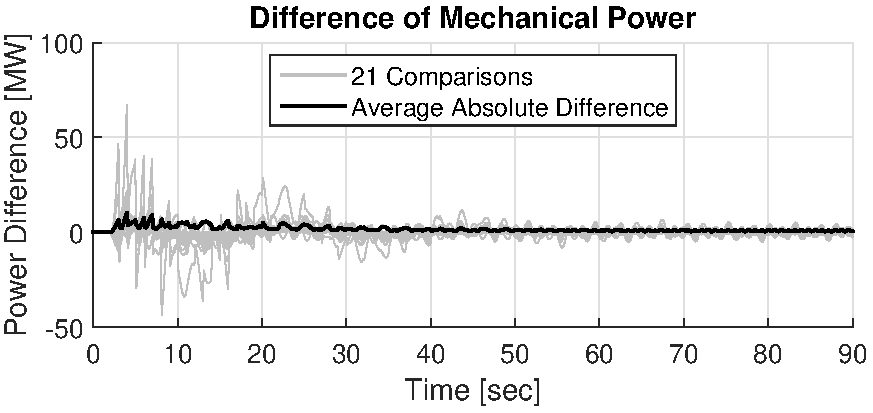
\includegraphics[width=\linewidth]{figures/miniWECC3ALTDstepPm2}
	\caption{Difference of mechanical power output during load step.}
	\label{fig: stepPmdif}
\end{figure}

\begin{figure}[!ht]
	\centering
	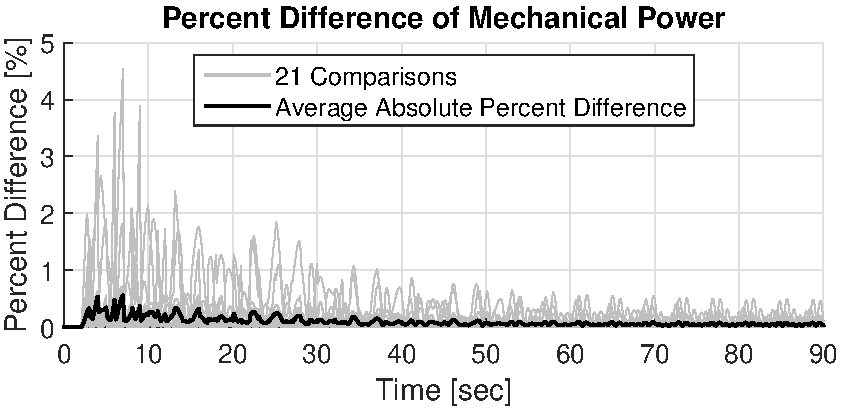
\includegraphics[width=\linewidth]{figures/miniWECC3ALTDstepPm3}
	\caption{Percent difference of mechanical power output during load step.}
	\label{fig: stepPmPercentdif}
\end{figure}


%`````````````````````````````````````````````````````````````````````````````````````
\subsubsection{Load Ramp Results}
Simulation results from a 40 second 400 MW load ramp, in Fig. \ref{fig: rampFcomp}-\ref{fig: rampPmdif} show frequency of LTD being within 1.2 mHz of PSDS and mechanical power differences of less than $\pm$10 MW or 1\% difference max (0.2\% average).
%*** Ramp results are included for now, but may be take up too much space... They do function as a `better' validation...

\begin{figure}[!ht]
	\centering
	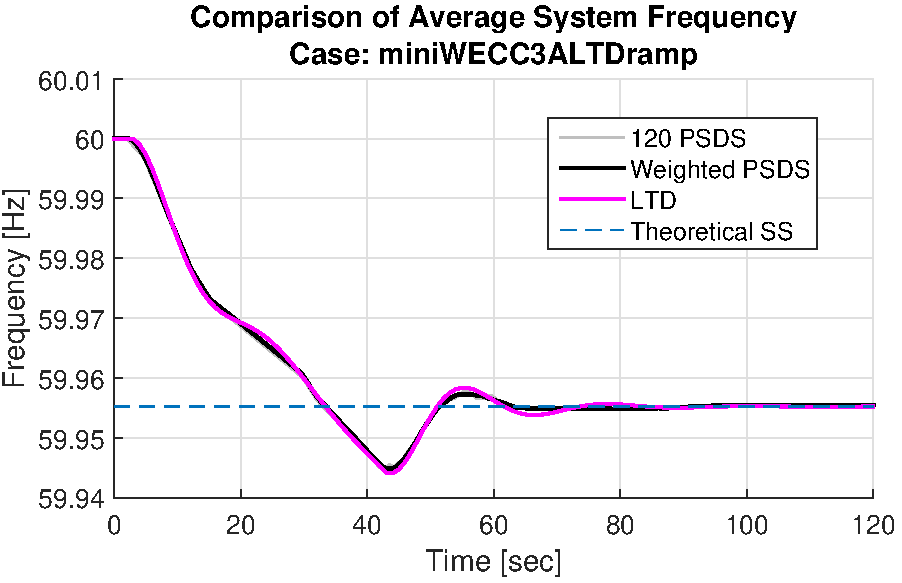
\includegraphics[width=\linewidth]{figures/miniWECC3ALTDrampF3}
	\caption{Comparison of frequency during load ramp.}
	\label{fig: rampFcomp}
\end{figure}

\begin{figure}[!ht]
	\centering
	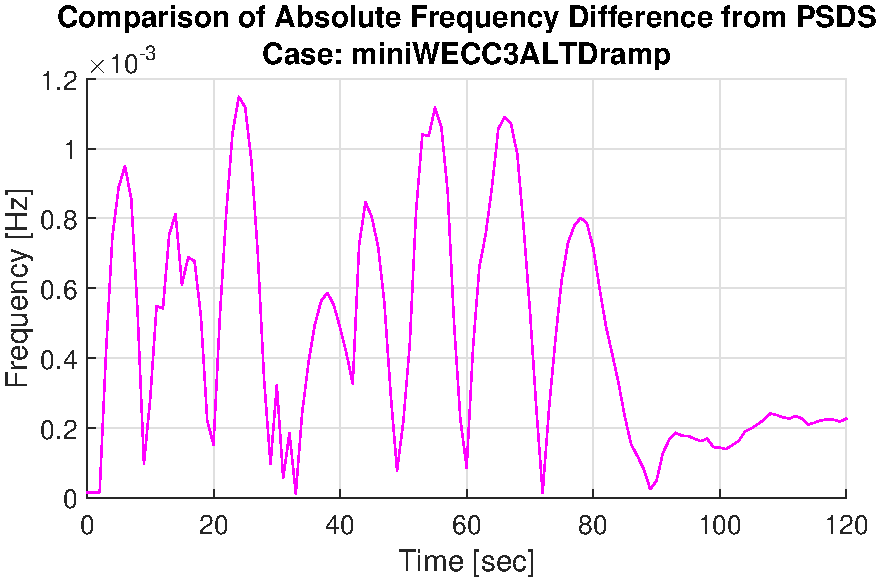
\includegraphics[width=\linewidth]{figures/miniWECC3ALTDrampRelF}
	\caption{Absolute difference of weighted frequency during load ramp.}
	\label{fig: rampFdif}
\end{figure}

\begin{figure}[!ht]
	\centering
	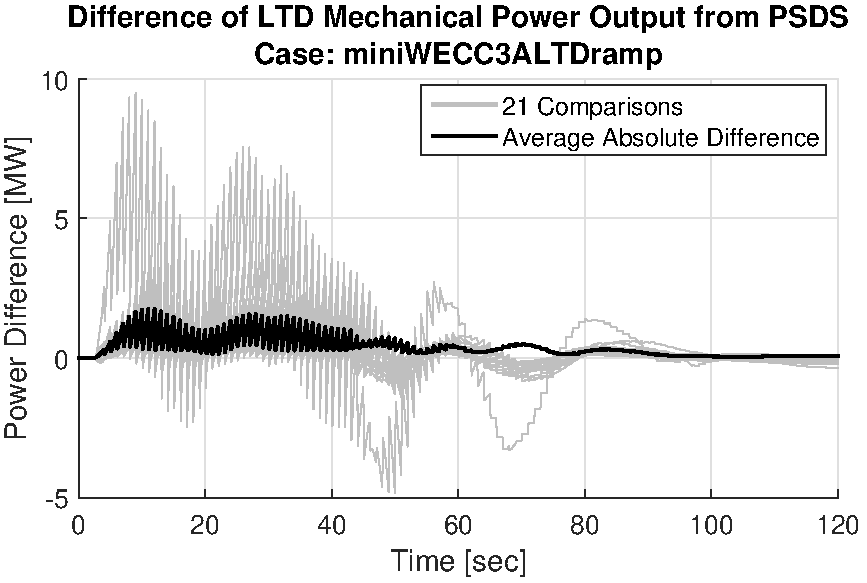
\includegraphics[width=\linewidth]{figures/miniWECC3ALTDrampPm2}
	\caption{Difference of mechanical power output during load ramp.}
	\label{fig: rampPmdif}
\end{figure}

\begin{figure}[!ht]
	\centering
	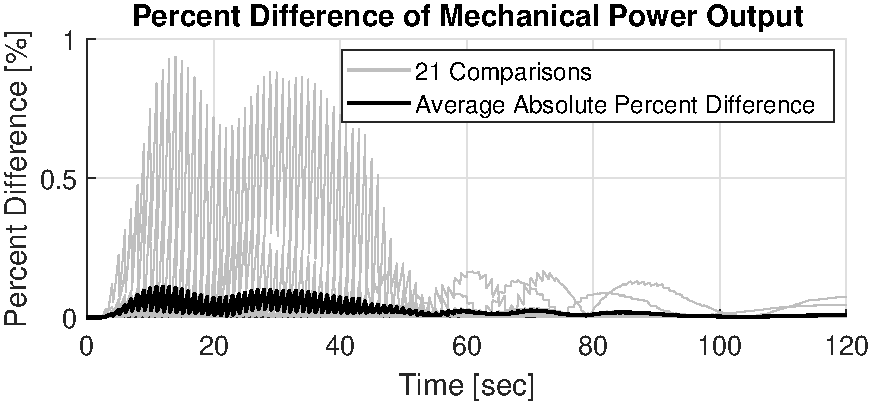
\includegraphics[width=\linewidth]{figures/miniWECC3ALTDrampPm3}
	\caption{Percent difference of mechanical power output during load ramp.}
	\label{fig: rampPmPercentdif}
\end{figure}
%-------------------------------------------------------------------------------------
\subsection{Validation Summary}
The step tests show the software is not meant to simulate large transient events with great accuracy.
However, small perturbances are modeled with less deviation from transient simulation methods.